% !TEX root = ../dg.tex

\section{The Differential}

In multivariable calculus, any differentiable map $f \from \R^m \to \R^n$ has a corresponding differential $df$.\footnote{You may have encountered this under the name \emph{Jacobian} rather than \emph{differential}; in the case $n=1$, this is [more or less] the gradient of the function.} While in a multivariable calculus setting we often think of $df$ as a map $\R^m \to \R^n$ as well (meaning it would have the same domain and codomain as $f$), or even more concretely as an $n \times m$ matrix, this is misleading.

In fact, if you were reading the first sentence of the previous paragraph very carefully, you may have noticed that it was not quite correct. Really, I should have said that any differentiable map has a corresponding differential \emph{at a point} $p$. There is no single ``differential'' for a non-linear map: we get different differentials in the neighborhood of each point in the domain.

So more accurately, if $p$ is in the domain of $f$, then we have a differential $df_p$ at $p$. Now, what is the domain of $df_p$? Recall, $df_p$ is supposed to be the best linear approximation of $f$ at $p$, so we're supposed to think of the inputs to $df_p$ as being slight perturbations of $p$. In other words, the domain of $df_p$ is really the tangent space $T_p \R^m$ (which is in a very precise sense the space of \emph{infinitesimal} perturbations of $p$).

Now, $T_p \R^m$ is isomorphic to $\R^m$, but not just in some abstract sense: the tangent bundle $T\R^m$ is trivial, meaning that $T \R^m \cong \R^m \times \R^m$, and a concrete trivialization is given by parallel translating a tangent vector from being based at $p$ to being based at the origin. This is the sense in which we can think of the domain of each $df_p$ as being the ``same'' $\R^m$.

But if $M$ is some more general $m$-dimensional manifold, then, while any tangent space $T_p M$ is still abstractly isomorphic to $\R^m$, the tangent bundle is likely not to be trivial, so we can't make any general identifications of different tangent spaces with the same $\R^m$. So if we want to generalize the notion of differential to manifolds, we need to be careful, even when thinking about functions on $\R^m$, to maintain the distinction between $\R^m$ (thought of an $m$-dimensional manifold) and $T_p \R^m$.

And what about the codomain of $df_p$? Again, we should think more conceptually about what the differential really does. Like all derivatives, the differential tells us something about how the change in an input to a function changes the output of the function. So the inputs to the differential will be tangent vectors at some point in the domain of $f$ (recording an infinitesimal change to the input, or equivalently an initial position [the point] and velocity [the tangent vector] of some path), and the outputs will be tangent vectors at the corresponding point in the range (recording the infinitesimal change in the output). Notice that $T_q \R^n$ is again isomorphic with $\R^n$ by parallel translation.

In other words, given a differentiable map $f \from \R^m \to \R^n$ and a point $p$ in the domain of $f$, the differential of $f$ at $p$ is a map $df_p \from T_p \R^m \to T_{f(p)}\R^n$, where domain and range are usually identified with $\R^m$ and $\R^n$ in a standard way. This, then, is the way of thinking about differentials which generalizes.

\begin{definition}\label{def:differential}
	Suppose $M^m$ and $N^n$ are smooth manifolds and $f \from M \to N$ is smooth. For each $p \in M$, define the \emph{differential} of $f$ at $p$, denoted $df_p\from T_p M \to T_{f(p)}N$, as follows: For any $v \in T_p M$, choose a smooth curve $\alpha \from (-\epsilon, \epsilon) \to M$ such that $\alpha(0) = p$ and $\alpha'(0) = v$. Let $\beta = f \circ \alpha$, which is a smooth curve in $N$. Then
	\[
		df_p(v) := \beta'(0).
	\]
\end{definition}

\begin{lemma}\label{lem:differential is well defined}
	This is a well-defined linear map.
\end{lemma}

\begin{exercise}
	Prove \cref{lem:differential is well defined}.
\end{exercise}

Let's see what this means in local coordinates, which is how we'll actually compute in practice. Suppose $p \in M$ and $(V, \psi)$ is a local coordinate chart on $N$ containing $f(p)$. By \cref{def:differentiable}, there exists some compatible chart $(U, \phi)$ on $M$ containing $p$ so that $f(\phi(U)) \subseteq \psi(V)$. Then the curve $\alpha$ on $M$ (or, really, its restriction to $\phi(U)$) gives a corresponding curve
\[
	(x_1(t), \dots , x_m(t)) = \phi^{-1} \circ \alpha(t)
\]
in $U \subseteq \R^m$, and similarly the curve $\beta$ on $N$ has a corresponding curve
\[
	(y_1(t), \dots , y_n(t)) = \psi^{-1} \circ \beta(t).
\]
See \cref{fig:differential}.

\begin{figure}[htbp]
	\centering
		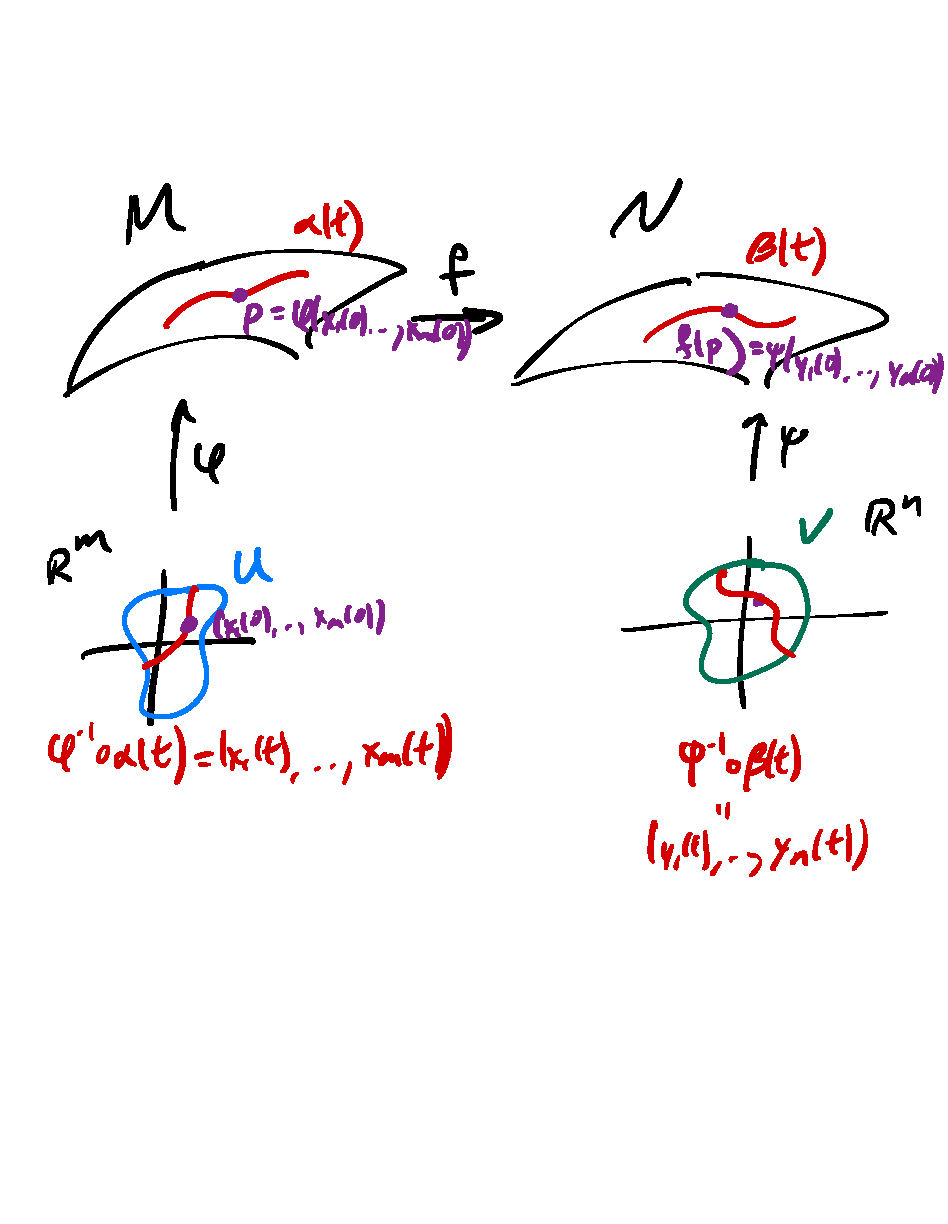
\includegraphics[height=2.5in]{differential}
	\caption{The differential in local coordinates}
	\label{fig:differential}
\end{figure}

Of course,
\[
	\psi^{-1} \circ \beta(t) = \psi^{-1} \circ f \circ \alpha(t) = \psi^{-1} \circ f \circ \phi(x_1(t), \dots , x_m(t)),
\]
so we can think of the $y_i$ as functions of the $x_j$, and the curve in $V$ can be written as
\[
	(y_1(x_1(t),\dots , x_m(t)), \dots , y_n(x_1(t), \dots , x_m(t))).
\]

Working in local coordinates means doing the computation at the level of the map $\psi^{-1} \circ f \circ \phi \from U \subseteq \R^m \to V \subseteq \R^n$, which has a corresponding differential
\[
	d(\psi^{-1} \circ f \circ \phi)_{(x_1(0),\dots , x_m(0))} \from T_{(x_1(0),\dots , x_m(0))} \R^m \to T_{(y_1(0), \dots , y_m(0))} \R^n.
\]
By definition, evaluating this differential on the tangent vector $(x_1'(0), \dots , x_m'(0)) \in T_{(x_1(0),\dots , x_m(0))}\R^m$ gives
\begin{align*}
	\left. \frac{d}{dt} \right|_{t=0} (y_1(x_1(t),\dots , x_m(t)), \dots , y_n(x_1(t),\dots , x_m(t))) & = \left( \sum_{j=1}^m \left.\frac{\partial y_1}{\partial x_j}\right|_{x} \left.\frac{d x_j}{dt} \right|_{t=0}, \dots , \sum_{j=1}^m \left.\frac{\partial y_n}{\partial x_j} \right|_x \left. \frac{d x_j}{dt} \right|_{t=0} \right) \\
	& = \left( \sum_{j=1}^m \left.\frac{\partial y_1}{\partial x_j}\right|_{x} x_j'(0), \dots , \sum_{j=1}^m \left.\frac{\partial y_n}{\partial x_j} \right|_x x_j'(0) \right) \\
	& = \begin{bmatrix} \frac{\partial y_1}{\partial x_1} & \cdots & \frac{\partial y_1}{\partial x_m} \\ \vdots & \ddots & \vdots \\ \frac{\partial y_n}{\partial x_1} & \cdots & \frac{\partial y_n}{\partial x_m} \end{bmatrix} \begin{bmatrix} x_1'(0) \\ \vdots \\ x_m'(0) \end{bmatrix} \\
	& = \begin{bmatrix} \frac{\partial y_i}{\partial x_j} \end{bmatrix}_{i,j} x'(0),
\end{align*}
where $\begin{bmatrix} \frac{\partial y_i}{\partial x_j} \end{bmatrix}_{i,j} $ is the $n \times m$ matrix of partials (i.e., the Jacobian).

So when we work in local coordinates, this is just standard multivariable calculus, as you would hope.

Just to reiterate, the differential (at a point) of a map between manifolds is going to input a tangent vector at a point in the domain and output a tangent vector at a point in the range. As a special case, suppose we have a smooth function on a manifold $M$; that is, a smooth map $f \from M \to \R$. Then, at a point $p \in M$, the differential $df_p \from T_p M \to T_{f(p)}\R$. Now, the tangent bundle to $\R$ is trivial, so we can identify $T_{f(p)}\R$ with $\R$ in a canonical way, and therefore think about $df_p$ as a linear map $T_pM \to \R$.

In other words, by way of this identification of $T_{f(p)} \R$ with $\R$, we can think of $df_p$ as a linear functional on the vector space $T_pM$. Or, in fancier language, $df_p$ is an element of the dual space $\left(T_pM\right)^\ast$. We'll come back to this later when we start talking about differential forms, but this gives a hint of why we might care about cotangent spaces and the cotangent bundle.

Just as in multivariable calculus, when we have a smooth map $f \from M \to N$, we can talk about critical points and critical values, and doing so is often quite important.

\begin{definition}\label{def:critical points}
	Let $f \from M \to N$ be smooth. A point $p \in M$ is a \emph{critical point} of $f$ if $df_p\from T_p M \to T_{f(p)}N$ is not surjective; then $f(p)$ is a \emph{critical value} of $f$. A point $q \in N$ which is not a critical value is a \emph{regular value} of $f$.
\end{definition}

\begin{example}[Cliché Example]
	Consider the function $f$ on the torus depicted in \cref{fig:morse-torus}. In words, $f$ is the height function on this upright torus that just records the $z$-coordinate. I've shown the critical values in red, as well as a couple of regular values in green. Also, back on the torus I've shown the inverse images of the critical and regular values, as well as some tangent vectors to regular points and their images under the differential (in blue and purple), to hopefully convince you the differential really is surjective at these points.
	
	\begin{figure}[htbp]
		\centering
			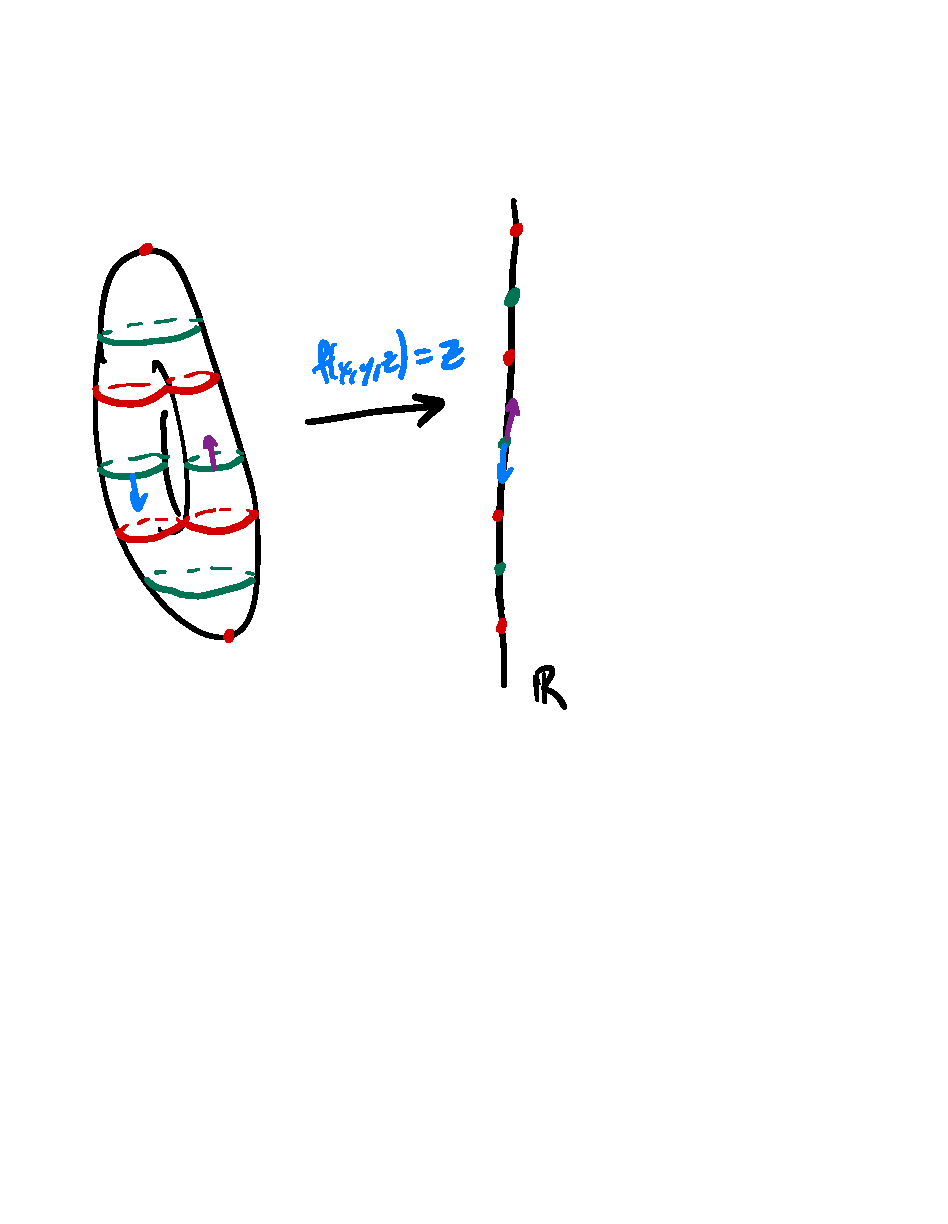
\includegraphics[height=3in]{morse-torus}
		\caption{The height function on a torus.}
		\label{fig:morse-torus}
	\end{figure}
	
	Notice that there are basically three different types of critical points: a minimum, a maximum, and two saddle points. The differential can't possibly be surjective at a (local) minimum: there's no direction you could go which will cause the function to decrease, so the image of the differential has to miss an entire half of its codomain (and therefore, by linearity, everything except the origin). It's somewhat less geometrically clear that the saddle points are critical points, though in this case it's fairly easy to see once you realize the tangent plane to one of the saddle points is horizontal.
	
	A couple of other things to notice about this picture:
	\begin{enumerate}
		\item The inverse images of the two critical points coming from the saddle points contain plenty of regular points: indeed, the differential is surjective at any of the points in the inverse image \emph{except} the saddle point.
		
		\item The level sets of regular values are smooth (collections of) curves, either a single circle or two disjoint circles; in other words, they are smooth (possibly disconnected) 1-dimensional manifolds. The level sets of the critical points are either a single point (the minimum and maximum) or a wedge of two circles (like an $\infty$ symbol). In both cases, the result is not a smooth 1-manifold: a point is a 0-manifold and the wedge of two circles is not locally like a copy of $\R$ near the point where the two circles meet (which of course is exactly the saddle point).
	\end{enumerate}
\end{example}

\begin{remark}
	I call this a cliché example because it is the first picture everybody draws when they talk about Morse theory, which says that the topology of a manifold is in some sense encoded in the critical points of any sufficiently generic function on the manifold. Such functions are called \emph{Morse functions}, and the function in this example is a Morse function. In particular, Morse theory tells you that if you are traversing the manifold ``up'' according to a Morse function, the topology only changes when you pass a critical point. In this example, the topology changes from the empty set to a disk when we pass the minimum, then from a disk to a 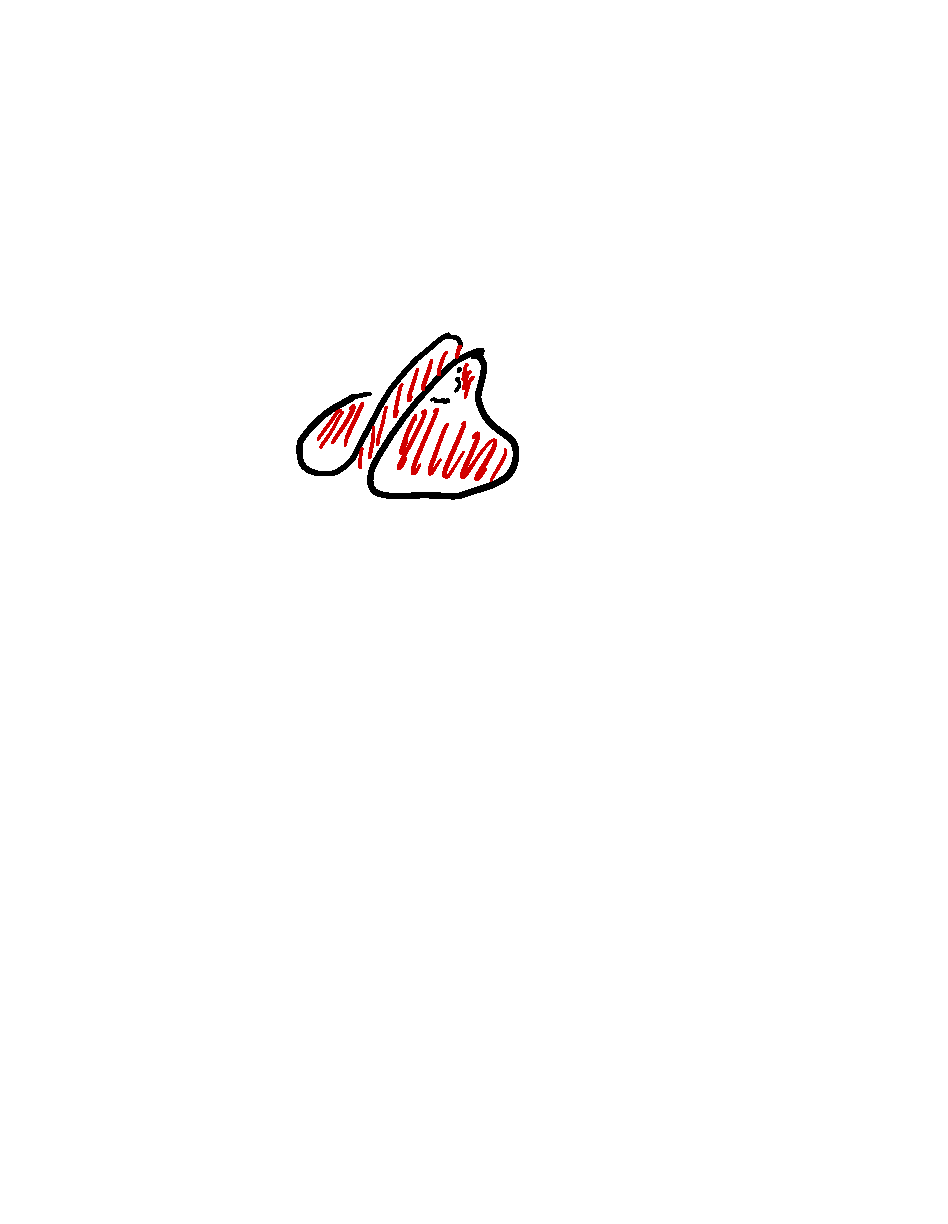
\includegraphics[height=.3in]{handle} (which is homotopic to a circle) when we pass the first saddle point, then to a punctured torus (which is homotopic to a wedge of circles) when we pass the second saddle point, and then finally the puncture is filled in when we pass the maximum. Something analogous happens in general.
\end{remark}

\begin{example}
	Consider the function $f(x,y,z) = z^2$ on the sphere (see \cref{fig:sphere}). Again, I've shown critical values in red and orange and a regular value in green, and the corresponding level sets on the domain, as well as some tangent vectors to regular points and their images under the differential.
	
		\begin{figure}[htbp]
			\centering
				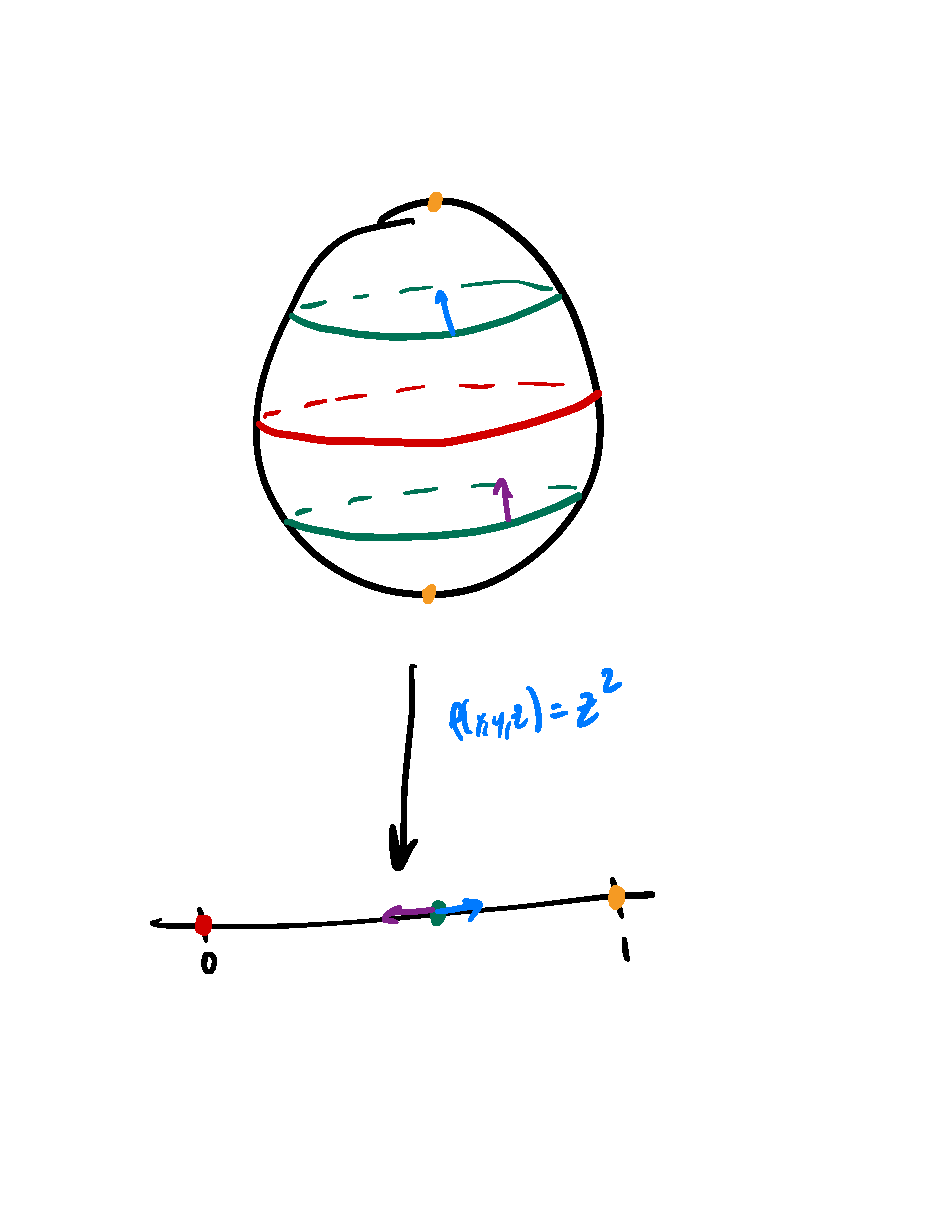
\includegraphics[height=2in]{morse-bott-sphere}
			\caption{A smooth function on the sphere which does not have isolated critical points.}
			\label{fig:sphere}
		\end{figure}
	
	Some new features:
	\begin{enumerate}
		\item The critical points aren't all isolated: the entire equator consists of critical points (which are all global minima).
		
		\item The inverse images of critical values aren't necessarily connected: the north and south poles both map to 1.
	\end{enumerate}
	
	Notice again that the level sets of regular values are (collections of) smooth curves. In this case one critical level set is also a smooth curve, and the other is not a curve at all.
	
	(This is not a Morse function because not all critical points are isolated, but it is a \emph{Morse–Bott function}, which is almost as good.)
	\end{example}
	
	After looking at these examples, hopefully the following theorem suggests itself:
	
	\begin{theorem}[Level Set Theorem]\label{thm:level set theorem}
		If $m \geq n$, $f \from M^m \to N^n$ is smooth, and $q \in N$ is a regular value of $f$, then $f^{-1}(q)$ is a smooth submanifold of $M$ of dimension $m-n$.
	\end{theorem}
	
	This theorem is basically an application of the Inverse Function Theorem, but before we work on proving it, let's look at some more examples.
	
	\begin{example}
		Define $f \from \R^n \to \R$ by $f(x_1,\dots , x_n) = x_1^2 + \dots + x_n^2$. Then
		\[
			df_{(x_1, \dots , x_n)}= \begin{bmatrix} \frac{\partial f}{\partial x_1} & \cdots & \frac{\partial f}{\partial x_n} \end{bmatrix} = \begin{bmatrix} 2x_1 & \cdots & 2x_n \end{bmatrix}
		\]
		only fails to be full rank at the origin, so 0 is the only critical value, and for all $r > 0$ the level set $f^{-1}(r)$ is a smooth manifold of dimension $n-1$. But $f^{-1}(r)$ is nothing but the sphere of radius $\sqrt{r}$, so we've just given an alternative (and somehow conceptually prior) proof that spheres are manifolds.
	\end{example}
	
	\begin{example}[Relevant to frame theory]
		Let $\Mat_{d \times N}(\C)$ be the space of $d \times N$ complex matrices. This is trivially a $2dN$-dimensional manifold, since $\Mat_{d \times N} (\C) \cong \C^{dN}$, which is just a copy of $\R^{2dN}$ if you ignore the complex structure. Now, let $\mathcal{H}(d)$ be the space of $d \times d$ Hermitian matrices (i.e., $d \times d$ complex matrices $A$ so that $A^\ast = A$, where $A^\ast$ is the conjugate transpose of $A$) and define the map $\Phi\from \Mat_{d \times N}(\C) \to \mathcal{H}(d)$ by
		\[
			\Phi(A) = A A^\ast.
		\]
		(In frame theory, we would think of $A \in \Mat_{d \times N}(\C)$ as a frame and $A A^\ast$ as the corresponding frame operator.)
		
		I claim that the identity matrix $I_{d \times d} \in \mathcal{H}(d)$ is a regular value of $\Phi$ (\textbf{Exercise:} Prove this); assuming this, the theorem tells us that $\Phi^{-1}(I_{d \times d})$ is a smooth manifold of dimension
		\[
			2dN - d^2 = d(2N-d).
		\]
		
		(Notice that $A \in \Phi^{-1}(I_{d \times d})$ means that the rows of $A$ are Hermitian orthonormal. Since each row is a vector in $\C^N$, this means that we can think of $\Phi^{-1}(I_{d \times d})$ as the space of all [ordered] $d$-tuples of Hermitian orthonormal vectors in $\C^N$. This space is an example of a \emph{Stiefel manifold}, and usually denoted $\operatorname{St}_d(\C^N)$ or $V_d(\C^N)$. In frame theory, $\Phi^{-1}(I_{d \times d})$ is precisely the space of \emph{Parseval frames}.)
	\end{example}
	
	\begin{example}\label{ex:U(d) manifold}
		Let $N=d$ in the previous example. Then $\Phi^{-1}(I_{d \times d})$ is a smooth manifold of dimension $d^2$ that consists of those $d \times d$ complex matrices $A$ so that $AA^\ast = I_{d \times d}$. But this is precisely the unitary group $\U(d)$! So we've proved that $\U(d)$ is a $d^2$-dimensional manifold for any $d$.
	\end{example}
	
	\begin{remark}
		You can play the same game over $\R$ to show that real Stiefel manifolds and the orthogonal group $\operatorname{O}(d)$ are manifolds.
	\end{remark}
